\section[Background]{Background \textnormal{\cite{Eichler_2018}}}

Lasers are ubiquitous tools of modern physics due to their useful properties, characterized by the emission of coherent light with narrow
spectral linewidth, low divergence and high power density. They are named after the acronym for light amplification by stimulated emission
of radiation, describing the fundamental mechanism for the production of laser radiation. This will be explored in the following, both in
the general as well as the special case of the \HeNe laser.

\subsection{Components of a laser}

The basic setup of a typical laser consists of three main components, namely an active medium, a pumping mechanism and the resonator cavity.

Inside the active medium, realized using materials such as semiconductors or gas mixtures, photons are emitted from atomic transitions to
energetically lower states. The energy difference $\Delta E$ between the involved electron levels is therefore the main determinant
of wavelength $\lambda$ and frequency $f$ via $\Delta E = hf$.

To excite electrons in the active medium to higher levels, an energy source is required. This is the role of the pumping mechanism, which
can be implemented using electrons or photons. The latter case is called optical pumping, as another separate light source tuned to the
respective $\Delta E$ value is used to induce transitions to excited states.

Amplification of the emitted radiation is achieved in the active medium. Instead of using superradiant lasers, which have high gain factors
and divergence, or impractically long constructions, mirrors can be used to create a resonator cavity. The resulting standing waves correspond
to multiple passes through the material and can generate a stable beam with low divergence, which can exit through a semitransparent window.
The mirror geometry can be adapted to the desired function with flat or concave designs.

\subsection{Processes in the active medium}

There are three main processes shown in Figure \ref{fig:processes} occuring inside the active medium to facilitate the operation of a laser.

\begin{figure}[H]
	\centering
	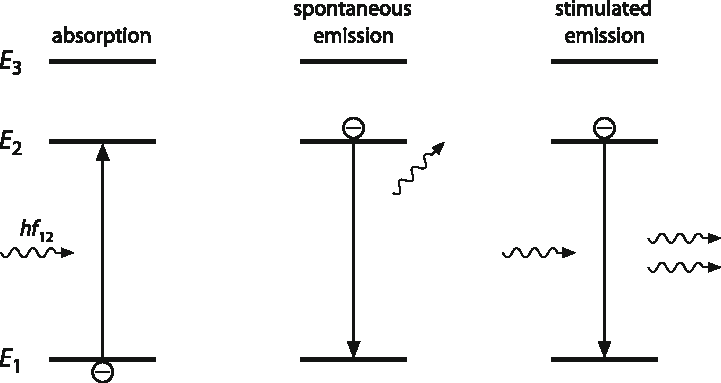
\includegraphics[width=0.65\textwidth]{content/graphics/processes.pdf}
	\caption{Schematic depiction of relevant processes inside the active medium. \cite{Eichler_2018}}
	\label{fig:processes}
\end{figure}

Raising the energy of an electron by $\Delta E = E_2 - E_1$ requires the annihilation of an incident photon that fulfills the condition
\begin{equation*}
	\Delta E = hf_{12} \: ,
\end{equation*}
where $h$ is the Planck constant. This process is referred to as absorption. The number of transitions per time and volume is proportional
to the density of ground state electrons $N_1$ as well as the photon flux or number per area and time $\varphi$ via
\begin{equation*}
	\left. \frac{dN_1}{dt} \right|_\text{ab} = -\sigma_{12} N_1 \varphi \: ,
\end{equation*}
with $\sigma_{12}$ denoting the effective cross section for absorbing a photon. From this also follows the typical exponential intensity
reduction
\begin{equation*}
	\left. \frac{dI}{dx} \right|_\text{ab} = -\sigma_{12} N_1 I \: ,
\end{equation*}
where $\alpha = -\sigma_{12} N_1$ gives the absorption coefficient.

When an atom is in an excited state, it returns to the ground state after a time interval, the duration of which follows some random
distribution with mean lifetime $\tau$. Due to its stochastic nature, this process is called spontaneous emission. The density in the
higher level then follows
\begin{equation*}
	\left. \frac{dN_2}{dt} \right|_\text{sp} = - \tau^{-1} N_2 \: .
\end{equation*}

Besides this, emission can also be initiated by an incoming photon of appropriate frequency. This is calles stimulated emission and results
in the production of radiation with the same energy, direction and phase as the inducing quantum. As the inverse process to absorption,
\begin{equation*}
	\left. \frac{dN_2}{dt} \right|_\text{st} = -\sigma_{21} N_2 \varphi \: ,
\end{equation*}
describes the time derivative and
\begin{equation*}
	\left. \frac{dI}{dx} \right|_\text{st} = \sigma_{21} N_2 I \: ,
\end{equation*}
the corresponding intensity relation.



\subsection{Necessity of multiple level systems}

\begin{figure}[H]
	\centering
	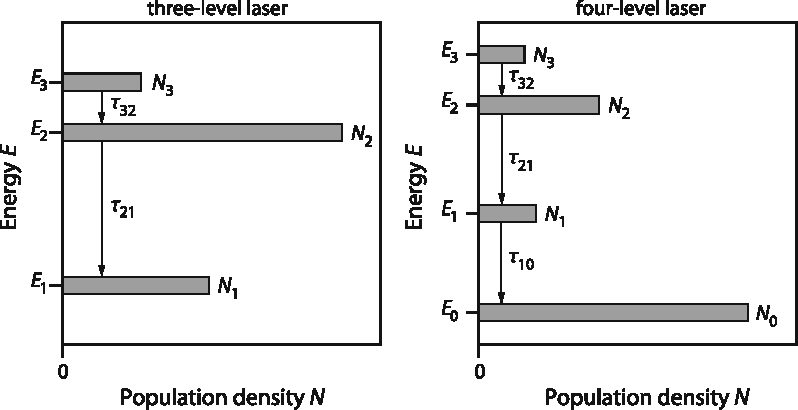
\includegraphics[width=0.70\textwidth]{content/graphics/levels.pdf}
	\caption{Exemplary energies and population densities for multiple levels. \cite{Eichler_2018}}
	\label{fig:processes}
\end{figure}

\subsection{Stability for different resonators}

\subsection{Transverse and longitudinal modes}

\subsection{Doppler broadening of the transition}

\subsection{Brewster windows and polarization}
